\subsubsection{XCSR}
\index{XCSR}
Wilson extended his concept of XCS with XCSR in \cite{WilsonXCSR}.
Classifier systems had typically taken strings from some small alphabet, often binary, as input until then
even though many real-world problems have input from the environment of the form $\mathbb{R}^n$ for some order $n \in \mathbb{Z}, n>0$.
Wilson's XCSR allows XCS to operate on just such an input.
XCSR is identical to normal XCS with the exception of the input interface, the nature of the predicates, the mutation operator, and the details of covering.
The basic structure of an XCSR rule is graphically illustrated in Figure~\ref{fig:xcsr-rule}.

Originally the predicates in XCSR were intervals of the form
\begin{equation}
interval_i = \{center_i,spread_i\},
\end{equation}
such that an environmental input $x_i$ was matched by $interval_i$ if and only if
\begin{equation}
center_i-spread_i \le x_i \le center_i+spread_i,
\end{equation}
but this was discovered to induce a bias \cite{StoneBull:2003}, so the representation was eventually changed to be
\begin{equation}
interval_i = \{lower_i,upper_i\},
\end{equation}
where now $x_i$ is matched by $interval_i$ if and only if
\begin{equation}
lower_i \le x_i \le upper_i.
\end{equation}
We use the $\{lower,upper\}$ form in this work.

\begin{figure}
\begin{center}
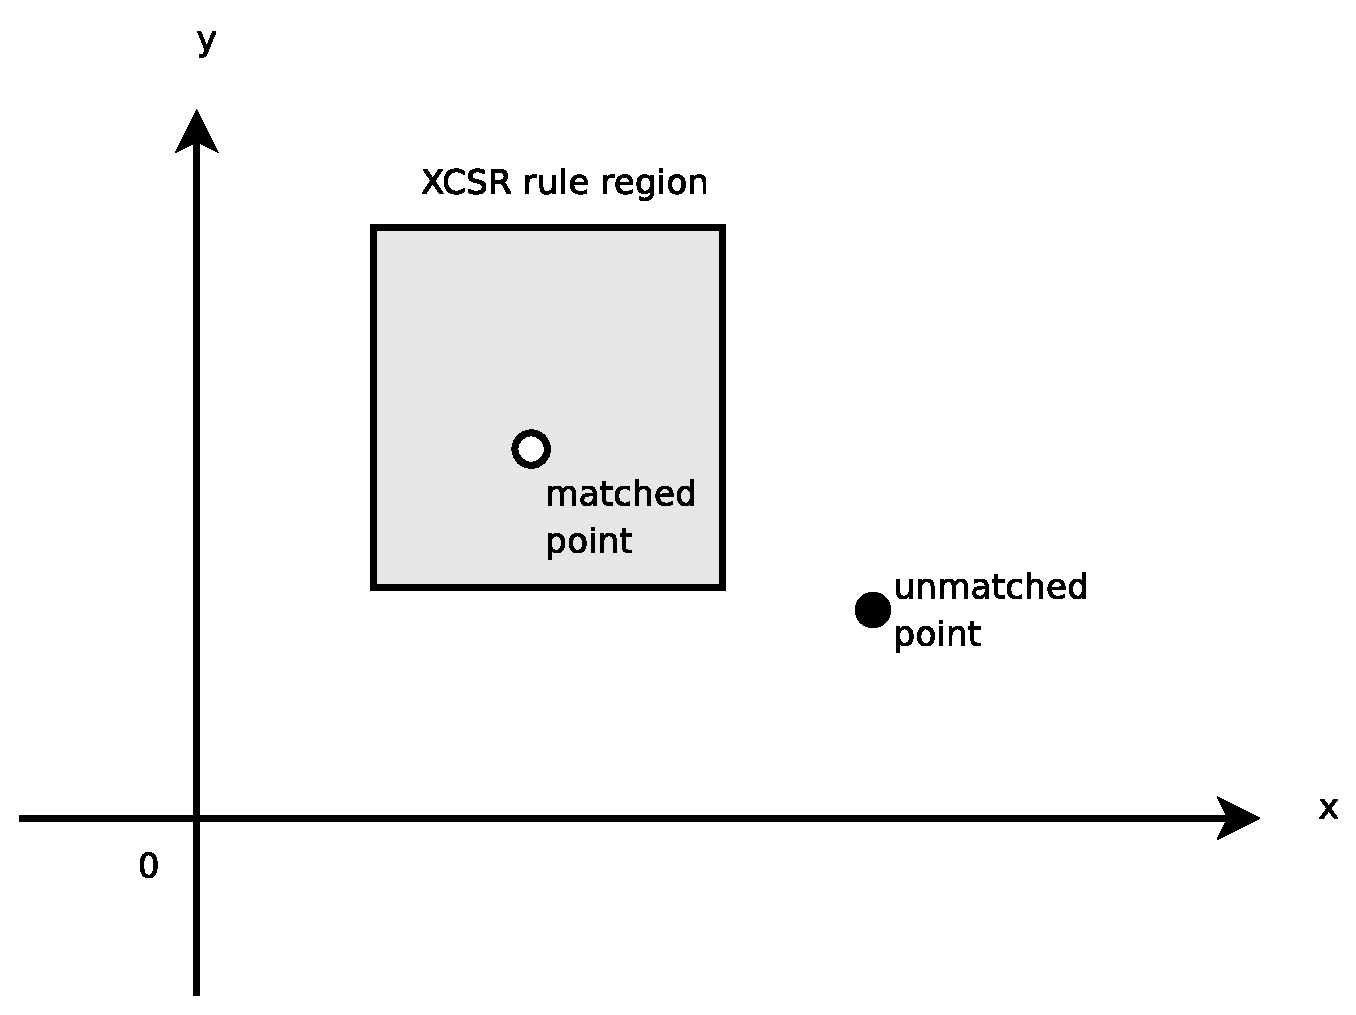
\includegraphics[width=4in]{xcsr-interval.eps}
\caption{XCSR's interval rules}
\label{fig:xcsr-rule}
\end{center}
\end{figure}

\newpage
Crossover is simple two-point crossover, but on the sequence
\begin{equation}
\{center_0,spread_0, \ldots\}
\end{equation}
or
\begin{equation}
\{lower_0,upper_0, \ldots\}
\end{equation}
depending on the predicate type,
in both cases therefore allowing the crossover points to fall within a single allele.

In the original XCSR, mutation was performed by adding a small random quantity from the range $[-0.1,0.1]$ to each allele, and all problems were to have their input scaled to $[0,1]$.
The variation of XCSR used here is capable of scaling outside of $[0.0,1.0]$, so instead mutation is performed as the addition or subtraction of a small percentage of the overall range as seen so far.
